%%%%%%%%%%%%%%%%%%%%%%%%%%%%%%%%%%%%%%%%%%%%%%%%%%%%%%%%%%%%%%%%%%%%%%
% Lớp 11 | Lý thuyết đồ thị | Bài toán tìm đường đi ngắn nhất
% Dạng 1C2?3-1: Bài toán tìm đường đi ngắn nhất
% Số câu: 9  (sinh tự động bởi tach_cau.py; từ nay thầy sửa trực tiếp file này)
%%%%%%%%%%%%%%%%%%%%%%%%%%%%%%%%%%%%%%%%%%%%%%%%%%%%%%%%%%%%%%%%%%%%%%

%%%%%%%%%%%%%%%% TRẮC NGHIỆM 4 PHƯƠNG ÁN %%%%%%%%%%%%%%%%

% nguồn: Ok_TracNghiemLop11_Lan1
\begin{ex}%[1C2B3-1]%[ma:6a42c1a5]
	Trong các dãy số $\left(u_n\right)$ cho bằng phương pháp truy  hồi sau, dãy số nào là cấp số nhân?
	\choice 
		{Dãy số $\left(u_n\right)$  được xác định bởi: $u_1=1$ và $u_n=u_{n-1}(n-1)$ với mọi $n \ge 2$}
		{Dãy số $\left(u_n\right)$ được xác  định bởi: $u_1=1$ và $u_n=2u_{n-1}+1$ với mọi $n \ge 2$}
		{Dãy số $\left(u_n\right)$ được xác định bởi: $u_1=1$  và $u_n={u_{n-1}}^2$ với mọi $n \ge 2$}
		{\True Dãy số $\left(u_n\right)$ được  xác định bởi: $u_1=3$ và $u_n=\dfrac{1}{3}u_{n-1}$ với mọi $n \ge 2$}
	 \loigiai{
		Dãy số  $\left(u_n\right)$ được xác định bởi: $u_1=3$ và $u_n=\dfrac{1}{3}u_{n-1}$ với mọi $n \ge 2$ là cấp số nhân.\\
		 Vì $\dfrac{u_n}{u_{n-1}}=\dfrac{1}{3}$ không đổi với mọi $n \ge 2$.
	} 
\end{ex}


%%%%%%%%%%%%%%%% TỰ LUẬN %%%%%%%%%%%%%%%%

% nguồn: Ok_TuanLuan_Toan11_Lan1
\begin{bt}%[1C2B3-1]%[ma:d02167be]
	Một quốc gia có dân số năm 2011 là $P$ triệu người. Trong $10$ năm tiếp theo, mỗi năm dân số tăng $a \%$. Chứng minh rằng dân số các năm từ năm 2011 đến năm 2021 của quốc gia đó tạo thành cấp số nhân.  Tìm công bội của cấp số nhân này.
	\loigiai{ 
		Coi  ngày điều tra dân số năm 2011 và năm 2021 trùng nhau thì từ năm 2011 đến năm 2021 là 10 năm. Vậy dân số nước ta tính đến năm 2021 là
		\[u_{10} = P\cdot  \left(1+a\%\right)^{10}.\]
		Ta có \[u_{1}  = P\cdot \left(1+a\%\right)^{1}.\]
		\[u_{2} = P\cdot  \left(1+a\%\right)^{2}.\]
		Và công bội của cáp số  nhân này là $\, \dfrac{u_2}{u_1} = q = \dfrac{P\cdot \left(1+a\%\right)^{2}}{P\cdot \left(1+a\%\right)^{1}} = 1+a\%.$
	 }
\end{bt}

% nguồn: Ok_TuanLuan_Toan11_Lan1
\begin{bt}%[1C2B3-1]%[ma:a9eefc78]
	Cho cấp số nhân $\left(u_n\right)$. Tìm số hạng đầu $u_1$, công bội  $q$ trong mỗi trường hợp sau:
	\begin{multicols}{2}
		\begin{enumerate}[a)]
			\item $u_6=192$ và  $u_7=384$;
			\item  $u_1+u_2+u_3=7$ và $u_5-u_2=14$.
		\end{enumerate}
	\end{multicols}
	\loigiai{ 
		\begin{enumerate}[a)]
			\item  $u_6=192$ và $u_7=384$;\\
			Ta có $\heva{u_6=192  \\ u_7=384} \Leftrightarrow \heva{u_1.q^5=192 \\ u_1.q^6=384} \Leftrightarrow \heva{u_1=6\\ q=2}$.\\
			Vậy số hạng  đầu $u_1=6$, công bội $q=2$.
			 \item $u_1+u_2+u_3=7$ và $u_5-u_2=14$.\\
			Ta có \begin{eqnarray*}
			&&\heva{u_1+u_2+u_3&=7  \\ u_5-u_2&=14} \Leftrightarrow \heva{u_1.(1+q+q^2)&=7 \\ u_1.q.(q^3-1)&=14} \Leftrightarrow \heva{u_1.(1+q+q^2)=7\\ q(q-1)=2} \\
			&\Leftrightarrow&  \heva{u_1.(1+q+q^2)=7\\ q^2-q-2=0.}\Leftrightarrow \hoac{\heva{u_1=1 \\ q=2}\\\heva{u_1&=7 \\ q&=-1.}}
		\end{eqnarray*}
		Vậy có  hai cấp số nhân thỏa mãn đề bài số hạng đầu $u_1=1$, công sai $q=2$; số hạng đầu $u_1=7$, công sai $q=-1$.
	\end{enumerate}
 }
\end{bt}

% nguồn: Ok_TuanLuan_Toan11_Lan1
\begin{bt}%[1C2Y3-1]%[ma:cbbcc6bb]
	Trong các dãy số sau,  dãy số nào là cấp số nhân? Vì sao?
	\begin{enumEX}[a)]{3}
		\item  $5$; $-0{,}5$; $0{,}05$; $-0{,}005$; $0{,}0005$;
		\item $-9$; $3$; $-1$;  $\dfrac{1}{3}$; $-\dfrac{1}{9}$;
		\item $2$; $8$; $32$; $64$;  $256$.
	\end{enumEX}
	 \loigiai{
		\begin{enumEX}[a)]{1}
			 \item Xét dãy số $5$; $-0{,}5$; $0{,}05$; $-0{,}005$; $0{,}0005$;
			Xét $q=\dfrac{-0{,}5}{5}=-\dfrac{1}{10}$. Ta có  \\
			$5q=-0{,}5$; $-0{,}5q=0{,}05$; $0{,}05q=-0{,}005$; $-0{,}005q=0{,}0005$. \\ 
			Vậy dãy số đã cho  là cấp số nhân với công bội $q=-\dfrac{1}{10}$.
			\item Xét dãy số $-9$; $3$; $-1$; $\dfrac{1}{3}$; $-\dfrac{1}{9}$;  Xét $q=\dfrac{3}{-9}=-\dfrac{1}{3}$. Ta có \\
			$-9q=3$;  $3q=-1$, $-1q=\dfrac{1}{3}$; $\dfrac{1}{3}q=-\dfrac{1}{9}$. \\
			Vậy dãy số đã cho là cấp số  nhân với công bội $q=-\dfrac{1}{3}$.
			\item Xét dãy số $2$; $8$; $32$; $64$; $256$. Xét  $q=\dfrac{8}{2}=4$. Ta có\\
			 $2q=8$; $8q=32$; $32q=128\neq 64$. \\
			Vậy  dãy số đã cho không phải cấp số nhân.
		\end{enumEX}
	} 
\end{bt}

% nguồn: Ok_TuanLuan_Toan11_Lan1
\begin{bt}%[1C2T3-1]%[ma:c8423b42]
	\immini{Cho hình vuông $C_1$ có cạnh bằng $4$. Người ta chia mỗi cạnh hình vuông thành bốn phần bằng nhau và nối các điểm chia một cách thích hợp để có hình vuông $C_2$ (\textit{Hình 4}). Từ hình vuông $C_2$ lại làm tiếp tục như trên để có hình vuông $C_3$. Cứ tiếp tục quá trình như trên, ta nhận được dãy các hình vuông $C_1, C_2, C_3, \ldots , C_n, \ldots$ Gọi $a_n$ là độ dài cạnh hình vuông $C_n$. Chứng minh rằng dãy số $\left(a_n\right)$ là  cấp số nhân.}{
	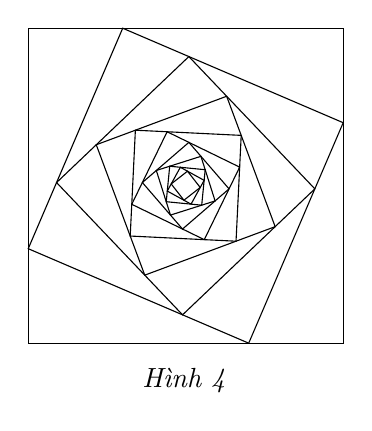
\begin{tikzpicture}
			 \def\a{2}
			\def\t{.7} 
			\path 
				(-\a,-\a)  coordinate (A1)
				(-\a,\a) coordinate  (B1)
				(\a,\a) coordinate (C1) 
				 (\a,-\a) coordinate (D1);
			\draw  (A1)--(B1)--(C1)--(D1)--cycle;
			\foreach  \i[count=\j from 2] in {1,...,10}
			 \draw
				(barycentric cs:A\i=\t,B\i=1-\t) coordinate  (A\j)--
				(barycentric cs:B\i=\t,C\i=1-\t) coordinate (B\j)-- 
				(barycentric cs:C\i=\t,D\i=1-\t) coordinate  (C\j)--
				(barycentric cs:D\i=\t,A\i=1-\t)  coordinate (D\j)--cycle;
			\node at  (0,-2.2) [below]{\textit{Hình 4}};
		\end{tikzpicture}
	 }
	\loigiai{ 
	\immini{Gọi cạnh một hình vuông thứ $n$, $n+1$ lần lượt là $a_n,  a_{n+1}$.\\
		Do $MN=\sqrt{MB^2+BN^2}=\sqrt{\left(\dfrac{AB}{4}\right)^2+\left(\dfrac{3AB}{4}\right)^2 }=AB.\dfrac{\sqrt{10}}{2}$.\\ 
		Nên  ta có cạnh hình vuông thứ $n+1$ là $a_{n+1}=a_n.\dfrac{\sqrt{10}}{2}$.\\
		Vậy dãy số $\left(a_n\right)$ là cấp số nhân.}{\begin{tikzpicture}[scale=0.8,>=stealth,font=\footnotesize,line join=round,line cap=round]
		 \tkzDefPoints{0/0/A,4/0/B}
		\tkzDefSquare  (A,B)\tkzGetPoints{C}{D}
		\tkzDrawPolygon  (A,B,C,D)
		\coordinate  (M) at ($(A)!0.75!(B)$);
		\coordinate (N) at ($(B)!0.75!(C)$); 
		 \coordinate (P) at ($(C)!0.75!(D)$);
		\coordinate (Q) at ($(D)!0.75!(A)$); 
		 \tkzDrawPolygon (M,N,P,Q)
		 \tkzLabelPoints[left](A,Q,D)
		\tkzLabelPoints[right](B,N,C) 
		 \tkzLabelPoints[below](M)
		\tkzLabelPoints[above](P) 
		 \tkzLabelSegment (A,B){$a_n$}
		 \tkzLabelSegment (M,N){$a_{n+1}$}
	\end{tikzpicture}
		} 
	 }
\end{bt}

% nguồn: Ok_TuanLuan_Toan11_Lan2
\begin{ex}%[1C2B3-1]%[ma:f1dce564]
	Một quốc gia có dân số năm 2011 là $P$ triệu người. Trong $10$ năm tiếp theo, mỗi năm dân số tăng $a \%$. Chứng minh rằng dân số các năm từ năm 2011 đến năm 2021 của quốc gia đó tạo thành cấp số nhân. Tìm công bội của cấp số nhân này. 
	 \loigiai{
		Coi ngày điều tra dân  số năm 2011 và năm 2021 trùng nhau thì từ năm 2011 đến năm 2021 là 10 năm. Vậy dân số nước ta tính đến năm 2021 là
		\[u_{10} = P\cdot \left(1+a\%\right)^{10}.\] 
		Ta có \[u_{1} = P\cdot  \left(1+a\%\right)^{1}.\]
		\[u_{2}  = P\cdot \left(1+a\%\right)^{2}.\]
		Và công bội của cáp số nhân này là $\,  \dfrac{u_2}{u_1} = q = \dfrac{P\cdot \left(1+a\%\right)^{2}}{P\cdot \left(1+a\%\right)^{1}} = 1+a\%.$
	 }
\end{ex}

% nguồn: Ok_TuanLuan_Toan11_Lan2
\begin{ex}%[1C2B3-1]%[ma:d7a0dee6]
	Cho  cấp số nhân $\left(u_n\right)$. Tìm số hạng đầu $u_1$, công bội $q$ trong mỗi trường hợp sau:
	\begin{multicols}{2}
		\begin{enumerate}[a)]
			 \item $u_6=192$ và $u_7=384$;
			\item $u_1+u_2+u_3=7$ và  $u_5-u_2=14$.
		\end{enumerate}
	\end{multicols}
	 \loigiai{
		\begin{enumerate}[a)]
			\item  $u_6=192$ và $u_7=384$;\\
			Ta có  $\heva{u_6=192 \\ u_7=384} \Leftrightarrow \heva{u_1.q^5=192 \\ u_1.q^6=384} \Leftrightarrow \heva{u_1=6\\ q=2}$.\\
			 Vậy số hạng đầu $u_1=6$, công bội $q=2$.
			\item $u_1+u_2+u_3=7$ và $u_5-u_2=14$.\\ 
			Ta có \begin{eqnarray*}
			&&\heva{u_1+u_2+u_3&=7 \\ u_5-u_2&=14} \Leftrightarrow \heva{u_1.(1+q+q^2)&=7 \\ u_1.q.(q^3-1)&=14}  \Leftrightarrow \heva{u_1.(1+q+q^2)=7\\ q(q-1)=2} \\
			 &\Leftrightarrow& \heva{u_1.(1+q+q^2)=7\\ q^2-q-2=0.}\Leftrightarrow \hoac{\heva{u_1=1 \\ q=2}\\\heva{u_1&=7 \\ q&=-1.}}
		\end{eqnarray*}
		Vậy có hai cấp số nhân thỏa mãn đề bài số hạng đầu $u_1=1$, công sai $q=2$; số  hạng đầu $u_1=7$, công sai $q=-1$.
	\end{enumerate}
 }
\end{ex}

% nguồn: Ok_TuanLuan_Toan11_Lan2
\begin{ex}%[1C2Y3-1]%[ma:f2f86f1b]
	Trong các dãy số sau, dãy số nào là cấp số  nhân? Vì sao?
	\begin{enumEX}[a)]{3}
		\item $5$; $-0{,}5$; $0{,}05$; $-0{,}005$; $0{,}0005$; 
		 \item $-9$; $3$; $-1$; $\dfrac{1}{3}$; $-\dfrac{1}{9}$;
		\item  $2$; $8$; $32$; $64$; $256$.
	\end{enumEX}
	 \loigiai{
		\begin{enumEX}[a)]{1}
			\item Xét dãy số $5$;  $-0{,}5$; $0{,}05$; $-0{,}005$; $0{,}0005$;
			Xét $q=\dfrac{-0{,}5}{5}=-\dfrac{1}{10}$. Ta  có \\
			$5q=-0{,}5$; $-0{,}5q=0{,}05$; $0{,}05q=-0{,}005$; $-0{,}005q=0{,}0005$. \\ 
			Vậy dãy số đã  cho là cấp số nhân với công bội $q=-\dfrac{1}{10}$.
			\item  Xét dãy số $-9$; $3$; $-1$; $\dfrac{1}{3}$; $-\dfrac{1}{9}$; Xét $q=\dfrac{3}{-9}=-\dfrac{1}{3}$. Ta có \\
			$-9q=3$;  $3q=-1$, $-1q=\dfrac{1}{3}$; $\dfrac{1}{3}q=-\dfrac{1}{9}$. \\
			Vậy dãy số đã cho là  cấp số nhân với công bội $q=-\dfrac{1}{3}$.
			\item Xét dãy số $2$; $8$; $32$; $64$; $256$. Xét $q=\dfrac{8}{2}=4$.  Ta có\\
			$2q=8$;  $8q=32$; $32q=128\neq 64$. \\
			Vậy dãy số đã cho không  phải cấp số nhân.
		\end{enumEX}
	 }
\end{ex}

% nguồn: Ok_TuanLuan_Toan11_Lan2
\begin{ex}%[1C2T3-1]%[ma:ea8c5ade]
	\immini{Cho hình vuông $C_1$ có cạnh  bằng $4$. Người ta chia mỗi cạnh hình vuông thành bốn phần bằng nhau và nối các điểm chia một cách thích hợp để có hình vuông $C_2$ (\textit{Hình 4}). Từ hình vuông $C_2$ lại làm tiếp tục như trên để có hình vuông $C_3$. Cứ tiếp tục quá trình như trên, ta nhận được dãy các hình vuông $C_1, C_2, C_3, \ldots , C_n, \ldots$ Gọi $a_n$ là độ dài cạnh hình vuông $C_n$. Chứng minh rằng dãy số $\left(a_n\right)$ là cấp số nhân.}{
	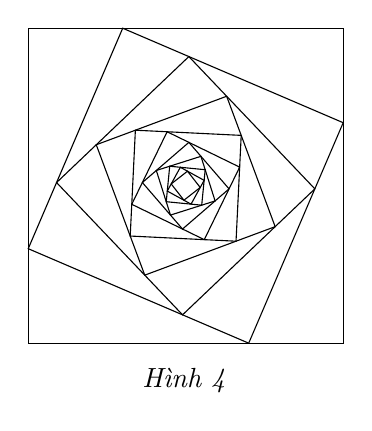
\begin{tikzpicture}
			\def\a{2} 
			 \def\t{.7}
			\path 
				(-\a,-\a)  coordinate (A1)
				(-\a,\a)  coordinate (B1)
				 (\a,\a) coordinate (C1)
				(\a,-\a) coordinate (D1); 
			\draw  (A1)--(B1)--(C1)--(D1)--cycle;
			\foreach \i[count=\j from 2] in {1,...,10} 
			 \draw
				(barycentric  cs:A\i=\t,B\i=1-\t) coordinate (A\j)--
				 (barycentric cs:B\i=\t,C\i=1-\t) coordinate (B\j)--
				(barycentric cs:C\i=\t,D\i=1-\t) coordinate  (C\j)--
				(barycentric cs:D\i=\t,A\i=1-\t) coordinate  (D\j)--cycle;
			\node at (0,-2.2)  [below]{\textit{Hình 4}};
		\end{tikzpicture}
	 }
	 \loigiai{
	\immini{Gọi cạnh một hình vuông thứ $n$, $n+1$ lần lượt là $a_n, a_{n+1}$.\\ 
		Do $MN=\sqrt{MB^2+BN^2}=\sqrt{\left(\dfrac{AB}{4}\right)^2+\left(\dfrac{3AB}{4}\right)^2 }=AB.\dfrac{\sqrt{10}}{2}$.\\ 
		Nên ta có cạnh hình vuông thứ $n+1$ là  $a_{n+1}=a_n.\dfrac{\sqrt{10}}{2}$.\\
		Vậy dãy số $\left(a_n\right)$ là cấp số nhân.}{\begin{tikzpicture}[scale=0.8,>=stealth,font=\footnotesize,line join=round,line cap=round]
		 \tkzDefPoints{0/0/A,4/0/B}
		 \tkzDefSquare (A,B)\tkzGetPoints{C}{D}
		 \tkzDrawPolygon (A,B,C,D)
		\coordinate  (M) at ($(A)!0.75!(B)$);
		\coordinate  (N) at ($(B)!0.75!(C)$);
		\coordinate  (P) at ($(C)!0.75!(D)$);
		\coordinate (Q)  at ($(D)!0.75!(A)$);
		\tkzDrawPolygon (M,N,P,Q) 
		 \tkzLabelPoints[left](A,Q,D)
		 \tkzLabelPoints[right](B,N,C)
		 \tkzLabelPoints[below](M)
		 \tkzLabelPoints[above](P)
		\tkzLabelSegment (A,B){$a_n$} 
		\tkzLabelSegment (M,N){$a_{n+1}$} 
	\end{tikzpicture}
		 }
	 }
\end{ex}
